\UseRawInputEncoding
\documentclass[a4paper, 14pt]{extarticle}

% Поля
%--------------------------------------
\usepackage{geometry}
\geometry{a4paper,tmargin=2cm,bmargin=2cm,lmargin=3cm,rmargin=1cm}
%--------------------------------------


%Russian-specific packages
%--------------------------------------
\usepackage[T2A]{fontenc}
\usepackage[utf8]{inputenc} 
\usepackage[english, main=russian]{babel}
\usepackage{cmap}
%--------------------------------------

\usepackage{textcomp}

% Красная строка
%--------------------------------------
\usepackage{indentfirst}               
%--------------------------------------             


%Graphics
%--------------------------------------
\usepackage{graphicx}
\graphicspath{ {./images/} }
\usepackage{wrapfig}
%--------------------------------------

% Полуторный интервал
%--------------------------------------
\linespread{1.3}                    
%--------------------------------------

%Выравнивание и переносы
%--------------------------------------
% Избавляемся от переполнений
\sloppy
% Запрещаем разрыв страницы после первой строки абзаца
\clubpenalty=10000
% Запрещаем разрыв страницы после последней строки абзаца
\widowpenalty=10000
%--------------------------------------

%Списки
\usepackage{enumitem}

%Подписи
\usepackage{caption} 

%Гиперссылки
\usepackage{hyperref}

\hypersetup {
	unicode=true
}

%Рисунки
%--------------------------------------
\DeclareCaptionLabelSeparator*{emdash}{~--- }
\captionsetup[figure]{labelsep=emdash,font=onehalfspacing,position=bottom}
%--------------------------------------

\usepackage{tempora}
\usepackage{amsmath}
\usepackage[dvipsnames]{xcolor}
\usepackage{listings}
\lstset{
  belowcaptionskip=1\baselineskip,
  breaklines=true,
  frame=L,
  xleftmargin=\parindent,
  language=Java,
  showstringspaces=false,
  basicstyle=\footnotesize\ttfamily,
  keywordstyle=\bfseries\color{blue},
  commentstyle=\itshape\color{purple},
  identifierstyle=\color{black},
  stringstyle=\color{red},
  numbers=left,           
  numberstyle=\tiny\color{gray}, 
  numbersep=10pt,      
  % ------------------------------
}

%--------------------------------------
%			НАЧАЛО ДОКУМЕНТА
%--------------------------------------

\begin{document}

%--------------------------------------
%			ТИТУЛЬНЫЙ ЛИСТ
%--------------------------------------
\begin{titlepage}
\thispagestyle{empty}
\newpage


%Шапка титульного листа
%--------------------------------------
\vspace*{-60pt}
\hspace{-65pt}
\begin{minipage}{0.3\textwidth}
\hspace*{-20pt}\centering

\includegraphics[width=\textwidth]{emblem}
\end{minipage}
\begin{minipage}{0.67\textwidth}\small \textbf{
\vspace*{-0.7ex}
\hspace*{-6pt}\centerline{Министерство науки и высшего образования Российской Федерации}
\vspace*{-0.7ex}
\centerline{Федеральное государственное бюджетное образовательное учреждение }
\vspace*{-0.7ex}
\centerline{высшего образования}
\vspace*{-0.7ex}
\centerline{<<Московский государственный технический университет}
\vspace*{-0.7ex}
\centerline{имени Н.Э. Баумана}
\vspace*{-0.7ex}
\centerline{(национальный исследовательский университет)>>}
\vspace*{-0.7ex}
\centerline{(МГТУ им. Н.Э. Баумана)}}
\end{minipage}
%--------------------------------------

%Полосы
%--------------------------------------
\vspace{-25pt}
\hspace{-35pt}\rule{\textwidth}{2.3pt}

\vspace*{-20.3pt}
\hspace{-35pt}\rule{\textwidth}{0.4pt}
%--------------------------------------

\vspace{1.5ex}
\hspace{-35pt} \noindent \small ФАКУЛЬТЕТ\hspace{80pt} <<Информатика и системы управления>>

\vspace*{-16pt}
\hspace{47pt}\rule{0.83\textwidth}{0.4pt}

\vspace{0.5ex}
\hspace{-35pt} \noindent \small КАФЕДРА\hspace{50pt} <<Теоретическая информатика и компьютерные технологии>>

\vspace*{-16pt}
\hspace{30pt}\rule{0.866\textwidth}{0.4pt}
  
\vspace{11em}

\begin{center}
\Large {\bf Летучка № 4} \\ 
\large {\bf по курсу <<Языки и методы программирования>>} \\ 
\large <<Модель вселенной>>
\end{center}\normalsize

\vspace{8em}


\begin{flushright}
  {Студент группы ИУ9-21Б Воронков А. С.\hspace*{15pt} \\
  \vspace{2ex}
  Преподаватель Посевин Д. П.\hspace*{15pt}}
\end{flushright}

\bigskip

\vfill
 

\begin{center}
\textsl{Москва 2026}
\end{center}
\end{titlepage}
%--------------------------------------
%		КОНЕЦ ТИТУЛЬНОГО ЛИСТА
%--------------------------------------

\renewcommand{\ttdefault}{pcr}

\setlength{\tabcolsep}{3pt}
\newpage
\setcounter{page}{2}

\section{Задание}
Реализовать модель вселенной. Каждый элемент вселенной должен быть объектом некоего публичного класса, который инициализируется вспомогательным публичным классом порождающим эту вселенную.
\begin{enumerate}
    \item 2	Реализовать вычисление среднего вектора направления движения частиц вселенной
    \item Вычислить силу притяжения действующую на произвольную частицу массой M находящейся в заданной координате пространства со стороны всех частиц вселенной
\end{enumerate}
\section{Практическая реализация}
Код файла Body.java
\begin{lstlisting}
import java.lang.Math;
import java.util.Date;

public class Body {
    String name;
    private final double x, y, z, v1, v2, v3, m;
    static Date timeStart;
    Date timeStartObj;

    static {
        timeStart = new Date();
    }

    public Body(String name, double x, double y, double z,
                double v1, double v2, double v3, double m) {
        this.name = name;
        this.x = x;
        this.y = y;
        this.z = z;
        this.v1 = v1;
        this.v2 = v2;
        this.v3 = v3;
        this.m = m;
        timeStartObj = new Date();
    }

    public Body(String name, double x, double y, double z) {
        this.name = name;
        this.x = x;
        this.y = y;
        this.z = z;
        v1 = (10000 + 10000) * Math.random() - 10000;
        v2 = (10000 + 10000) * Math.random() - 10000;
        v3 = (10000 + 10000) * Math.random() - 10000;
        m = 1000000000 * Math.random();
        timeStartObj = new Date();
    }


    public Body(String name) {
        this.name = name;
        x = (100 + 100) * Math.random() - 100;
        y = (100 + 100) * Math.random() - 100;
        z = (100 + 100) * Math.random() - 100;
        v1 = (10000 + 10000) * Math.random() - 10000;
        v2 = (10000 + 10000) * Math.random() - 10000;
        v3 = (10000 + 10000) * Math.random() - 10000;
        m = 1000000000 * Math.random();
        timeStartObj = new Date();
    }

    public double getX() {return x;}
    public double getY() {return y;}
    public double getZ() {return z;}
    public double getV1() {return v1;}
    public double getV2() {return v2;}
    public double getV3() {return v3;}
    public double getM() {return m;}

    public String gtTime() {
        return String.valueOf(timeStartObj.getTime() - timeStart.getTime());
    }
}
\end{lstlisting}
\par
Код файла Universe.java
\begin{lstlisting}
import java.util.Date;

public class Universe {
    Body[] parts;
    int ln;
    static Date timeStart;
    Date timeStartObj;
    final double G = 6.67 * Math.pow(10, -11);

    static {
        timeStart = new Date();
    }

    public Universe(int n) {
        parts = new Body[n];
        ln = 0;
        timeStartObj = new Date();
    }

    public void addPart(Body... objs) {
        for (Body obj : objs) {
            if (ln == parts.length) {
                System.out.println("University overflowed");
                return;
            }
            parts[ln] = obj;
            ln++;
        }
    }

    public double[] getMeanV() {
        int n = parts.length;
        double sumV1, sumV2, sumV3;
        sumV1 = sumV2 = sumV3 = 0;
        for (Body obj : parts) {
            sumV1 += obj.getV1();
            sumV2 += obj.getV2();
            sumV3 += obj.getV3();
        }
        double v1 = sumV1/n, v2 = sumV2/n, v3 = sumV3/n;
        double norm = Math.sqrt(Math.pow(v1, 2) + Math.pow(v2, 2) + Math.pow(v3, 2));
        return new double[]{v1/norm, v2/norm, v3/norm};
    }

    public double getF(Body obj) {
        double f1, f2, f3, f;
        double m = obj.getM();
        double x = obj.getX();
        double y = obj.getY();
        double z = obj.getZ();
        f1 = f2 = f3 = 0;
        double dx, dy, dz, r;
        for (Body i : parts) {
            dx = x - i.getX();
            dy = y - i.getY();
            dz = z - i.getZ();
            r = Math.sqrt(Math.pow(dx, 2) + Math.pow(dy, 2) + Math.pow(dz, 2));
            if (r == 0) {continue;}
            f = G * m * i.getM() / Math.pow(r, 2);
            f1 += f * dx / r;
            f2 += f * dy / r;
            f3 += f * dz / r;
        }
        return Math.sqrt(Math.pow(f1, 2) + Math.pow(f2, 2) + Math.pow(f3, 2));
    }

    public String gtTime() {
        return String.valueOf(timeStartObj.getTime() - timeStart.getTime());
    }
}
\end{lstlisting}
\par
Код файла Main.java
\begin{lstlisting}
import java.util.Arrays;

public class Main {
    public static void main(String[] args) {
        int n = 5;
        Universe universe = new Universe(n);
        System.out.println("Время до инициализации вселенной: " + universe.gtTime());
        for (int i = 0; i < n; i++) {
            universe.addPart(new Body(String.valueOf(i)));
            System.out.println("Время до инициализации частицы " + i
                    + " " + universe.parts[i].gtTime());
        }

        double[] meanV = universe.getMeanV();
        System.out.printf("Средний вектор направления: %.2f %.2f %.2f\n",
                meanV[0], meanV[1], meanV[2]);

        System.out.printf("Сила притяжения действующая на частицу %.2f Ньютонов",
                universe.getF(new Body("test", 5.0, -45.0, 34)));
    }
}

\end{lstlisting}

\begin{center}
    \nopagebreak
    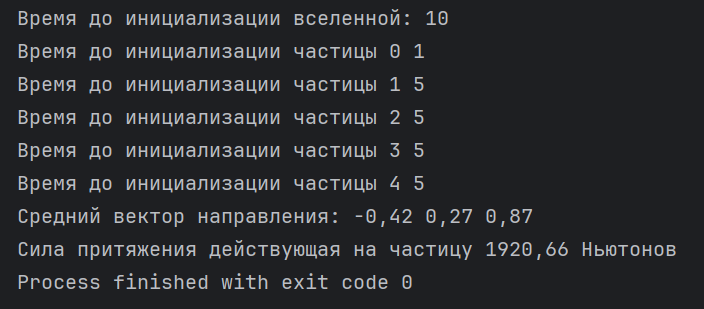
\includegraphics[width=0.85\textwidth]{let4_1}
    \captionsetup{justification=centering}
    \captionof{figure}{Результат работы Main.java}
\end{center}

\section{Вывод}
В данной летучке были получены навыки работы со static блоками. Была создана модель вселенной с объектами класса частиц вселенной
\end{document}